\chapter{Servidor Local}\label{ch:servidor}

	\section{¿Que es un Servidor Loca?}
	
	Un servidor local se refiere a una computadora que se mantiene encendida y conectada a una red LAN de manera constante. Su función principal consiste en proporcionar una variedad de servicios y contenidos a través de dicha red, sin importar el dispositivo que los usuarios utilicen. Al no requerir acceso directo por parte de los usuarios, no es necesario contar con un monitor ni un teclado conectados a esta computadora.
		
	\section{Uso del servidor}
	
El servidor local ofrece servicios de alojamiento de archivos y streaming. Estos servicios permiten a los usuarios almacenar y acceder a archivos de manera remota, así como transmitir contenido multimedia a través de la red local. El servidor local despliega su capacidad para gestionar y distribuir eficientemente estos servicios, brindando a los usuarios la posibilidad de compartir y acceder a sus archivos y contenido multimedia de manera conveniente y segura.		
		
		\begin{itemize}

\item\textbf{Servidor de archivos:} permite alojar, sincronizar y compartir archivos con otros usuarios y dispositivos conectados a la misma red. Al almacenar los archivos localmente, proporciona un control total sobre los datos, asegurando la privacidad y permitiendo un acceso rápido y eficiente a los archivos compartidos.

\item\textbf{Servidor Streaming:} se encarga de gestionar el contenido multimedia, como música, películas, series y documentales. Este servicio permite reproducir dicho contenido en cualquier dispositivo conectado a la misma red, brindando una experiencia de entretenimiento fluida y accesible.

Ambos servicios del servidor local trabajan en conjunto para facilitar el intercambio y la reproducción de archivos y contenido multimedia dentro de la red local, ofreciendo comodidad y flexibilidad a los usuarios.\par
		
		\end{itemize}
		
	\section{Sistema Operativo}
				
			Por las características propias de Debian no necesitare buscar un sistema operativo orientado a 	servidores, dado que me permitirá crear un potente servidor, al poseer estabilidad/escalabilidad y buenos repositorios.\par
		
	\section{Instalación del Sistema Operativo}\label{install}
			
		Una vez que comience el proceso de instalación, seguiré una serie de pasos que me permitirán instalar y configurar el sistema operativo :
		
		\begin{itemize}
			
			\item \textbf{Graphical Install}
			
			\item \textbf{Localización:} Seleccionar el idioma de instalación que será el idioma utilizado por el sistema. (Por motivos de compatibilidad, se recomienda seleccionar English) Después indicar la localización geográfica del servidor.
			
			\item \textbf{Configure Locale:} Seleccionar “United Estates” para evitar conflictos de compatibilidad.
			
			\item \textbf{Configuración del teclado:} Seleccionar Spanish o Latin America.
			
			\item \textbf{Conexión a Internet:} Para conectarse a Internet se necesita la asignación de una dirección IP a la interfaz de red. La dirección IP y los demás parámetros de la red pueden obtenerse de forma automática a partir de un servidor DHCP o se pueden configurar manualmente.
			
			\item \textbf{Nombre del sistema:} Nombre con el que se conocerá al sistema en la red.
			
			\item \textbf{Cuentas de usuario y passwords:} El programa instalador solicita la creación y configuración de dos cuentas de usuario del sistema o logins. La primera es la cuenta de root y la segunda es una cuenta de usuario ‘normal’, con permisos limitados.
			
			\item \textbf{Reloj del sistema y huso horario:} El instalador intentará sincronizar el reloj del sistema con uno de los servidores que establecen la hora oficial en el Internet.
			
			\item \textbf{Particionado:} Por fines prácticos creare un LVM y seleccionare el método guiado para usar todo el disco. Luego Gestionare el GV de la siguiente manera:
			
			GNU/Linux tiene un nivel de personalización muy amplio, es por ello, que seguramente no todos verán necesario lo que realizare, así como quizás haya alguien que piense que hay muchos otros directorios más susceptibles que no se mencionan y deben alojarse en un (LV).
			
			La gestión de volúmenes consistirá en organizar la raíz del sistema en varios volúmenes. Cada uno de estos pueden tener un objetivo y/o un tipo de sistema de archivos distinto y específico. 
			
			A continuación mencionare los directorios que tendrán su propio (LV), dado el uso que le
			daré al servidor.	
			
			\vspace{0.3cm}

			
			\begin{itemize}
				
				\item \textbf{Directorio /var:} En este directorio se encontraran todo tipo de archivos, de los cuales se espera que en una ejecución normal del sistema estén cambiando continuamente. Estos podrían ser “logs, bases de datos, spool, cachés, e-mail, etc”. \par
									
				\item \textbf{Directorio /tmp:} En este directorio es donde las aplicaciones almacenarán archivos temporales. Tiene la particularidad de que siempre será borrado tras un reinicio del sistema.\par
				
				\item \textbf{Directorio /usr:} Es con frecuencia grande, debido a que todos los programas están instalados aquí. 
				
				\item \textbf{Directorio /srv:}	Sirve para almacenar archivos y directorios relativos a servidores.	
				
				\item \textbf{/var/lib/docker} Los volúmenes se almacenan en /var/lib/docker/volumes/. Docker almacena los datos dentro de este directorio. 
				
				\item \textbf{Directorio /home:} Es donde se crean los directorios de los usuarios normales.
				
				\item \textbf{Directorio /opt:} En este directorio se instalan algunos programas de terceros, además es el directorio donde suelo guardar ejecutables.
				
			\end{itemize}
			
			\item \textbf{Instalación del sistema base:} En este paso el instalador comenzará la instalación de los paquetes de aplicaciones necesarios para crear un sistema base. Este proceso puede tardar algún tiempo.
			
			\item \textbf{Configuración del gestor de paquetes apt:} Seleccionar el repositorio geográficamente más cercano al equipo que se está instalando. En primer lugar se debe elegir el país y luego escoger el mirror más próximo.
			
			\item \textbf{Concurso de popularidad:} La comunidad Debian mantiene un concurso de popularidad interno, con el fin de obtener estadísticas sobre los sistemas instalados. La instalación de este	paquete implica la instalación de otros paquetes. No se recomienda instalar el paquete de popularidad para que el sistema sea lo más ligero posible.
			
			\item \textbf{Finalizar instalación:} El instalador permite la instalación automática de diversas configuraciones del sistema. Como se busca personalizar totalmente el sistema, se anulará cualquier selección existente. De esta forma se instalará un sistema con un mínimo de funcionalidades.
			
			\item \textbf{Instalación del gestor de arranque grub:} En este punto el sistema ya está casi completamente instalado. Sin embargo, para que el sistema pueda arrancar hay que instalar el gestor de arran	que “grub” en el master boot record (mbr) del disco.
			Una vez instalado el grub se debe seleccionar continuar, y el equipo se reiniciara automática mente para el primer login.
		
		\end{itemize}
	
	\section{LVM}
	
		\subsection{¿Que es LVM?}
		
			LVM es una capa de abstracción entre un dispositivo de almacenamiento y un sistema de ficheros. Las ventajas que tienen son múltiples, pero la inicial y por la cual lo uso, es por la flexibilidad frente al particionado tradicional. Con LVM las limitaciones en el redimencionado y particionado desaparecen. Se puede aumentar el tamaño  de los volúmenes lógicos independientemente de que no haya espacio libre contiguo.
				
				\begin{itemize}
					
					\item \textbf{Volumen físico o Physical Volume (PV):} Un volumen físico es un dispositivo de bloque que se le entregará al LVM para que este lo gestione.
					
					\item \textbf{Grupo de volúmenes o Volume Group (VG):} Para poder usar el espacio de almacenamiento de un PV, éste debe pertenecer a un Grupo de volúmenes. Un VG es una especie de disco duro virtual compuesto de uno o más PVs. 
					
					\item \textbf{Volumen Lógico o Logical Volume (LV):} Los volúmenes lógicos son dispositivos en los cuales se crea sistemas de archivos. Por seguir con la analogía del \textit{«disco duro virtual»} que es el VG, los LVs serían las particiones. 
					
				\end{itemize}
			
	
		\subsection{Gestión volúmenes lógicos}
		
			Los volúmenes lógicos son donde todos los datos se almacenan en un LVM. Para crear los nuevos volúmenes lógicos, utilizare los siguiente comandos.

			
			\begin{lstlisting}[language=Bash, caption=Creación de LV]
				
			lvcreate -L 10G -n home ema
			lvcreate -L 10G -n docker ema
			lvcreate -L 100G -n srv ema
			lvcreate -L 5G -n opt ema
			lvcreate -L 1G -n tmp ema
			lvcreate -L 15G -n usr ema
			lvcreate -L 1G -n var-tmp ema
			lvcreate -L 1G -n var-log ema
			lvcreate -L 2G -n swap ema
								
			\end{lstlisting}
		
			La sintaxis básica para crear volúmenes lógicos es:
			
			lvcreate \textbf{-L} \textit{«tamaño»}\textbf{G} \textbf{-n} \textit{«nombre del volumen»} \textit{«nombre del grupo»}
			
			\begin{itemize}
				
				\item \textbf{-L} Tamaño en GB o MB.
				\item \textbf{-n} Nombre que tendrá el (LV) Nombre del VG con el que se trabajara.
			 
			\end{itemize}
			
		
			Luego de que los (LVs) estén disponibles, les creare un sistema de archivo:
			
			\begin{lstlisting}[language=Bash, caption=Crear Sistema de Archivo]
						
			mkfs.ext4 /dev/mapper/ema-var--log
			mkfs.ext4 /dev/mapper/ema-var--tmp
			mkfs.ext4 /dev/mapper/ema-tmp
			mkfs.ext4 /dev/mapper/ema-opt
			mkfs.ext4 /dev/mapper/ema-home
			mkfs.ext4 /dev/mapper/ema-docker
			mkfs.ext4 /dev/mapper/ema-usr
			mkfs.ext4 /dev/mapper/ema-srv
			mkswap /dev/mapper/ema-swap
			
			\end{lstlisting}
			
			\vspace{0.3cm}
			
			Una vez creados los sistemas de archivo es hora montar los (LVs) y mover el contenido de los directorios al (LV) correspondiente.
			
			\begin{lstlisting}[language=Bash, caption=Crear directorios y montar los (LVs)]
				
			mv /mnt
			
			mkdir {var-log,opt,home,usr,srv}
			
			mount /dev/mapper/ema-var--log var-log
			mount /dev/mapper/ema-opt opt
			mount /dev/mapper/ema-home home
			mount /dev/mapper/ema-usr usr
			mount /dev/mapper/ema-srv srv
			
			\end{lstlisting}
			
			\vspace{0.3cm}
			
			Mover todo el contenido de los directorios a su	 (LV) correspondiente.
			
			\begin{lstlisting}[language=Bash, caption=Mover directorios]
			
			#Mover el contenido de los directorios
			mv -f var/log/* var-log
			mv opt/* opt
			mv -f home/* home
			mv usr/* usr
			mv srv/* srv
			#Eliminar archivos temporales
			rm -rf var/tmp/*
			rm -rf tmp/*
			
			\end{lstlisting}
		
		
		\section{fstab}
			
			El archivo /etc/fstab es el archivo de configuraciones que une dispositivos con punto de montaje. Le indica al sistema cómo montar cada dispositivo y qué configuración utilizar.\par
			
			Tabla de configuración del archivo fstab: 
			
			\begin{lstlisting}[language=Bash, caption=fstab]
					
			# <file system> <mount point> <type> <options> <dump> <pass>
			
			\end{lstlisting}
			
			\begin{itemize}
				 
				\item \textbf{file system:} Esta primera columna guarda el dispositivo a montar. 
				
				\item \textbf{mount point:}	Esta opción permite definir el directorio que se va a asociar con el (LV) definido en la primera columna. 
				
				\item \textbf{Tipo:} Este campo se refiere al tipo de filesystem, por ejemplo, ext4, xfs, entre otros.
				
				\item \textbf{Opciones:} Hace referencia a las opciones de montaje. Deben ir separadas por comas. 
				
				Algunas de las opciones que se pueden usar son:
				
				\begin{itemize}
				 	
					\item \textbf{auto:} para que la partición se monte al arrancar.
					
					\item \textbf{noauto:} opción que impide que la partición se monte durante el arranque.
					
					\item \textbf{user:} los usuarios tienen permitido montar la partición.
					
					\item \textbf{nouser:} solo el usuario root tiene permitido realizar el montaje de la partición.
					
					\item \textbf{ro:} partición que solo permite la lectura.
					
					\item \textbf{rw:} opción que permite la lectura escritura.
					
					\item \textbf{exec:} es posible ejecutar los binarios pertenecientes a esa partición.
					
					\item \textbf{async:} esta opción permite que el sistema continúe trabajando luego de una petición de escritura del equipo, aunque no haya recibido la confirmación.
				
					\item \textbf{suid:} esta opción permite las operaciones con los bits suid y sgid. Es utilizado para permitir a los usuarios diferentes del root, ejecutar binarios con ciertos privilegios otorgados temporalmente para que realicen una labor determinada.
					
					\item \textbf{nosui:} se encarga de impedir el funcionamiento de los bits suid y sgid.
					
					\item \textbf{noatime:} esta opción no actualiza el nodo-i de los ficheros con el tiempo de acceso. Además, permite aumentar las prestaciones del sistema, debido a que accede menos al disco.
					
					\item \textbf{nodiratime:} con esta opción se impide la actualización del nodo-i de los directorios con el tiempo de acceso. Al igual que la opción noatime, también puede aumentar las prestaciones del sistema.
				
					\item \textbf{defaults:} establece que las opciones sean asignadas por defecto gracias al sistema operativo. Estas opciones predeterminadas son  rw, suid, dev, exec, auto, nouser y async.
				
				\end{itemize}
	
				\item \textbf{Soporte a Dump:} Este campo es requerido por algunas soluciones de backup. Además, determina la frecuencia con la que debe realizarse la copia de seguridad.
				
				\item \textbf{Chequeo automático:} Es el campo encargado de especificar si el sistema de ficheros debe ser revisado durante el arranque, si el formato es correcto, entre otros. Normalmente ese campo se deshabilita para todas las particiones, a excepción del /.
				
			\end{itemize}
		
			\subsection{Configurar fstab}
			
				Es necesario que defina que los (LVs) se monten automáticamente cuando se está iniciando el sistema operativo. La forma correcta para resolver este problema es modificando el archivo fstab.
				
				Finalizada la configuración mi archivo fstab quedara de la siguiente manera:

				\vspace{0.3cm}
									
				\inputminted{bash}{documentos/fstab/fstab}
	
	\section{Controlar cambios en el sistema}
		
		Por cuestiones de seguridad tomo como buena practica generar HASH de los archivos que se encuentran en algunos directorios que considero importante, por si en algún momento tengo la duda de que se generaron cambios en el sistema, poder realizar las comparaciones de HASH.
	
		\clearpage
		
		\subsection{Generar Hash}
			
			md5sum es un algoritmo de reducción criptográfico de 128-bits desarrollado por MIT. Se utiliza con frecuencia como herramienta para validar un archivo.
			
			\inputminted{bash}{documentos/seguridad/generarHash.sh}
					
		
		\subsection{Comparar Hash}
			
			Si por alguna razon necesito validar la integridad de los archivos del sistema, utilizo el siguiente script en bash.
		
			\inputminted{bash}{documentos/seguridad/compararHash.sh}
			
	\section{Configuración de red}
	
		\subsection{Asignar una IP estática}
			
			El servidor tendrá una dirección IP estática, la cual se la asignare editando el archivo \textit{"interfaces"}.\par
			
			\begin{lstlisting}[language=Bash, caption=Interfaces]		
				nvim /etc/network/interfaces	
			\end{lstlisting}
			
			A continuación presento el contenido del archivo /etc/network/interfaces con una configuración de IP estática:
			
			\begin{lstlisting}[language=Bash, caption=Configuración de IP estática]	
				# This file describes the network interfaces available on your system
				# and how to activate them. For more information, see interfaces(5).	
				source /etc/network/interfaces.d/*
				# The loopback network interface
				auto lo
				iface lo inet loopback	
				# Interfaz de red enp2s0
				auto enp2s0
				allow-hotplug enp2s0
				iface enp2s0 inet static
					address   192.168.1.222
					netmask   255.255.255.0
					network   192.168.1.0
					broadcast 192.168.1.255
					gateway   192.168.1.1
			\end{lstlisting}
			
			\begin{itemize}
				
				\item \textbf{iface enp2s0 inet static:} define el nombre lógico de la interfaz de red enp2s0,
				la \textit{address\_family} que es \textbf{inet} y el método de configuración de la interfaz que es \textbf{static}.
				
				\item \textbf{address:} define la IP que tendrá el servidor.
			
				\item \textbf{netmask:} define la máscara de subred.
			
				\item \textbf{network:} define la dirección de red.
			
				\item \textbf{broadcast:} define la IP de difusión (broadcast).
			
				\item \textbf{gateway:} define la IP de la puerta de enlace (gateway).
			
			\end{itemize}
						
			Una vez finalizada la edición del archivo reiniciare el servicio de red para aplicar los cambios. \par
			
									
			\begin{lstlisting}[language=Bash, caption=Reiniciar servicio de RED]			
				systemctl restart networking.service
			\end{lstlisting}
			
		
		\subsection{Servidor DNS}
			
		
			Es necesario que tambien configure los servidores DNS. Para configurarlos editare el archivo /etc/resolv.conf:\par
	
		
			\begin{lstlisting}[language=Bash, caption=Editar archivo resolv]		
				nvim /etc/resolv.conf
			\end{lstlisting}
		
			
			A continuación presento el contenido del archivo /etc/resolv.conf con dos servidores DNS:

		
			\begin{lstlisting}[language=Bash, caption=Servidores DNS]	
			# Dynamic resolv.conf(5) file for glibc resolver(3) generated by resolvconf(8)
			#     DO NOT EDIT THIS FILE BY HAND -- YOUR CHANGES WILL BE OVERWRITTEN	
			nameserver 1.1.1.1    
			nameserver 8.8.8.8
			\end{lstlisting}
		

			\begin{itemize}
				
				\item \textbf{1.1.1.1:} Es un DNS público operado por Cloudflare que ofrece una forma rápida y privada de navegar por Internet. A diferencia de la mayoría de los servidores de DNS, 1.1.1.1 no vende los datos de los usuarios a los anunciantes.

				\item \textbf{8.8.8.8:} Como una forma de hacer más rápida la web Google tiene, Google Public DNS. Que es una forma de navegar fuera de los límites del proveedor de servicios de internet.

			\end{itemize}

				
	\section{Firewall}
		
		\subsection{¿Que es iptables?}
		
			Iptables es una herramienta de filtrado de paquetes en Linux. Se encarga de analizar cada uno de los paquetes del tráfico de red que entra en una máquina y decidir, en función de un conjunto de reglas, qué hacer con ese paquete.
			
			Gracias a la capacidad de analizar el tráfico y ver las características del paquete, se puede implementar un cortafuegos que controle qué paquetes puede llegar al equipo.
			
			\subsubsection{Características de iptables:}
			
				\begin{itemize}
					\item Es el sucesor de ipfwadm e ipchains, un software previo que existía en sistemas Linux.
				
					\item Se encuentra disponible desde la rama 2.4 del kernel de Linux, que se lanzó el año 2001.
				
					\item Está desarrollado por el proyecto netfilter. Este mismo proyecto ha desarrollado también el sucesor de iptables, que se denomina nftables, aunque en la actualidad todavía está mucho más extendido el uso de iptables que el de nftables.
					
				\end{itemize}		
			
			\subsection{Reglas iptables}
			
				El siguiente script en bash me permitirá configurar el el firewall de linux.
			
				\inputminted{bash}{documentos/firewall/firewall.sh}
	
			
	\section{Servidor Docker}
	
		\subsection{¿Que es Docker?}
			Docker es una plataforma de contenerización de código abierto. Permite a los desarrolladores empaquetar aplicaciones en contenedores. Los contenedores combinan el código fuente de la aplicación con las bibliotecas del sistema operativo y las dependencias necesarias para ejecutar el código en cualquier entorno. Los contenedores simplifican la entrega de aplicaciones distribuidas.\par
			Docker es esencialmente un kit de herramientas que permite a los desarrolladores crear, implementar, ejecutar, actualizar y detener contenedores utilizando comandos a través de una única API.
			
		\subsection{Funcionamiento de los contenedores?}
			Los contenedores son posibles gracias al aislamiento de procesos y a las capacidades de virtualización integradas en el kernel de Linux. Estas funcionan como grupos de control (Cgroups) para asignar recursos entre procesos, y espacios de nombres para restringir un acceso de procesos o visibilidad a otros recursos o áreas del sistema.\par	
			
			Como resultado, los contenedores ofrecen toda la funcionalidad y beneficios de las máquinas virtuales, incluyendo aislamiento de aplicaciones, escalabilidad y capacidad de disposición. Sus ventajas son las siguientes:\par
			
			\begin{itemize}
				\item \textbf{Ligero:} Los contenedores sólo incluyen los procesos y dependencias del sistema operativo necesarias para ejecutar el código.
				
				\item \textbf{Mejor manejo de los recursos:} Con contenedores se puede ejecutar varias veces las mismas copias de una aplicación en el mismo hardware.
				
				\item \textbf{Mayor productividad de los desarrolladores:} En comparación con las VM, los contenedores son más rápidos y fáciles de implementar, suministrar y reiniciar.
			
			\end{itemize}
			
		\subsection{Características}
		
			\vspace{0.3cm}
				
			\begin{itemize}
					
				\item \textbf{Portabilidad:} Los contenedores LXC suelen hacer referencia a 		configuraciones especificas de la máquina, mientras que los contenedores Docker se ejecutan sin modificaciones en cualquier entorno de escritorios, centro de datos y nube.
				
				\item \textbf{Ligeros:} Con los contenedores Docker solo se puede ejecutar un proceso en cada contenedor. Esto permite crear una aplicación que puede continuar ejecutándose mientras una de sus partes se desactiva.
									
				\item \textbf{Creación automática de contenedores:} Docker puede crear automáticamente un contenedor basado en el código de origen de la aplicación.
				
				\item \textbf{Control de versiones:} Docker puede rastrear versiones de una imagen de contenedor, retroceder a versiones anteriores y rastrear quién creó una versión. 
			
				\item \textbf{Reutilizar contenedores:} Los contenedores existentes se pueden utilizar como imágenes base, esencialmente como plantillas para crear nuevos contenedores.
				
				\item \textbf{Repositorio de contenedores:} Los desarrolladores pueden acceder a un registro de código abierto que contiene miles de contenedores aportados por los usuarios.
			
			\end{itemize}
			
		\subsection{Herramientas de Docker}
			
			\vspace{0.3cm}
			
			\begin{itemize}
					
				\item \textbf{DockerFile:} Cada contenedor Docker se inicia con un archivo de texto simple que contiene instrucciones para crear la imagen del contenedor Docker. El DockerFile es una lista de instrucciones de interfaz de línea de comandos que Docker Engine ejecutará para ensamblar la imagen.
				
				\item \textbf{Imágenes Docker:} Las imágenes Docker contienen el código de origen de la aplicación, herramientas, bibliotecas y dependencias que el código de la aplicación debe ejecutar como contenedor.\par
				
				Las imágenes Docker son archivos de sólo lectura.
				
				\item \textbf{Contenedores Docker:} Los contenedores Docker son las instancias activas en ejecución de imágenes Docker.\par
				 
				Los contenedores son contenido en vivo, efímero y ejecutable. Se pueden interactuar con ellos utilizando comandos Docker.
				
				\item \textbf{Docker Hub:} Es el repositorio público de imágenes Docker. Las imágenes de contenedor provienen de proveedores de software comercial, proyectos de código abierto y desarrolladores individuales. Ademas de las imágenes que han sido producidas por Docker, Inc.\par
				
				\item \textbf{Daemon Docker:} El daemon Docker es un servicio que se ejecuta en el sistema operativo. Este servicio crea y gestiona las imágenes Docker.
				

			\end{itemize}
		
		
		\subsection{Instalación Docker}
			
			\vspace{0.1cm}
			
			Antes de comenzar con la instalación es necesario que se instalen unas herramientas:
					
			\begin{itemize}
				
				\item\textbf{apt-transport-https:} permite que el administrador de paquetes transfiera datos a través de https.
				
				\item\textbf{ca-certificates:} permite que el navegador web y el sistema verifiquen los certificados de seguridad.
				
				\item\textbf{curl:} transfiere datos.
				
				\item \textbf{software-properties-common:} agrega scripts para administrar el software.
				
			\end{itemize}	
				
				
			\begin{lstlisting}[language=Bash, caption=Paquetes necesarios]
	#actualizar lista de paquetes
	apt update
	#instalar herramientas
	apt install curl apt-transport-https ca-certificates software-properties-common
	
			\end{lstlisting}
			
			\textbf{Clave GPG:}\par
			
			\begin{lstlisting}[language=Bash, caption=Clave GPG]
	#crear directorio
	mkdir -p /etc/apt/keyrings
	#descargar key
	curl -fsSL https://download.docker.com/linux/debian/gpg | gpg --dearmor -o /etc/apt/keyrings/docker.gpg
			\end{lstlisting}
		
			\textbf{Agrega el repositorio:}
	
			\begin{lstlisting}[language=Bash, caption=Repositorio]

	#agregar repositorio
	echo "deb [arch=$(dpkg --print-architecture) signed-by=/etc/apt/keyrings/docker.gpg] https://download.docker.com/linux/debian $(lsb_release -cs) stable" | sudo tee /etc/apt/sources.list.d/docker.list > /dev/null
			\end{lstlisting}
	
			\textbf{Instalar Docker Engine.}\par
	
	
			\begin{lstlisting}[language=Bash,caption=docker]
	#actualizar lista de paquetes
	apt update
	#instalar docker
	apt install docker-ce docker-ce-cli containerd.io docker-compose-plugins
			\end{lstlisting}


			Para verificar que docker se esta ejecutando correctamente ejecutare el contenedor de Hello-World, el cual da una bienvenida.
	
			\begin{lstlisting}[language=Bash,caption=Hello-World]
	#descargar y ejecutar contenedor de bienvenida
	docker run hello-world
			\end{lstlisting}
		
		\subsection{¿Que es Docker Compose?}
		
			Docker Compose es una herramienta que permite simplificar el uso de Docker a partir de un archivo YAML. De esta manera es mas sencillo crear contendores, conectarlos, habilitar puertos, volúmenes, etc.\par 
		
		\subsection{Instalación Docker Compose}
			
			\vspace{0.2cm}
			
			Hay varias versiones de Docker Compose, aunque siempre es preferible la versión estable.

									
			\begin{lstlisting}[language=Bash,caption=Docker Compose]
	#descargar binario de docker-compose	
	curl -L "https://github.com/docker/compose/releases/download/1.26.0/docker-compose-$(uname -s)-$(uname -m)" -o /usr/local/bin/docker-compose
	#cambiar permisos
	chmod +x /usr/local/bin/docker-compose
	#controlar la version de docker-compose
	docker-compose --version
			\end{lstlisting}
				
				
	\section{Contenedor NextCloud}
		
		\subsection{¿Que es Nextcloud?}
		
			Nextcloud es un servidor para el intercambio de archivos que permite almacenar contenido personal (documentos e imágenes, videos, etc) en una ubicación centralizada. Al ser sus funciones de código abierto, ofrece una gran versatilidad, seguridad y cumplimiento a las normas de privacidad. También permite aplicar diferentes políticas a los datos, como cifrado, administración de usuarios y auditoría.\par
		
	
			\subsection{Características:}
		
				\begin{itemize}
					
					\item Los archivos Nextcloud son almacenados en estructuras de directorio convencionales y se
					pueden acceder vía WebDAV.
					
					\item Los archivos son cifrados en la transmisión y opcionalmente durante el almacenamiento.
					
					\item Los usuarios pueden manejar calendarios CalDAV, contactos CardDAV, tareas programadas y
					reproducir contenido multimedia Ampache.
					
					\item Permite la administración de usuarios y grupos de usuarios, vía OpenID o LDAP y definir per-
					misos de acceso.
					
					\item Posibilidad de añadir aplicaciones de un solo clic y conexiones con Dropbox, Google Drive y
					Amazon S3.
					
					\item Disponibilidad de acceso a diferentes bases de datos, mediante SQLite, MariaDB, MySQL,
					Oracle Database, y PostgreSQL
					
					\item Cuenta con aplicaciones clientes para Windows, MAC OSX, Linux, Android y IOS.\par
					
					
				\end{itemize}

			\subsection{Requisitos:}
		
				
				Al ejecutarse dentro de un contenedor todas sus dependencias se encuentran resueltas, solo se debera considerar la cantidad de memoria RAM.\par
					
				La documentación de Nextcloud indica que la cantidad de memoria que se necesita para ejecutar un servidor Nextcloud es muy variable, y dependerá de la cantidad de usuarios, aplicaciones, archivos y volumen de actividad del servidor.\par
			
			\subsection{Preparación del área de trabajo}
				
				Mi directorio de trabajo sera \textit{/srv} donde creare un directorio que almacenara toda las configuraciones de Nextcloud, asi como la configuración de la base de datos.
				
				\begin{lstlisting}[language=Bash,caption=Directorio de trabajo NextCloud]
			#cambiar al directorio /srv
			cd /srv
			#crear directorio Nextcloud
			mkdir nextcloud
			#entrar al directorio Nextcloud
			cd nextcloud
				\end{lstlisting}
			
				Dentro del directorio creare un documento llamado \textit{docker-compose.yaml} y dentro de el colocare el siguiente código:
	
				\inputminted{yaml}{documentos/docker/nextcloud/docker-compose.yml}
			
				\subsubsection{Estructura del docker-compose.yml}\label{estructura-docker}
				
					\begin{itemize}
						
						\item \textbf{version:} Un archivo de docker-compose comienza especificando la versión de docker compose que se utilizará.
							
						\item \textbf{services:} Después de la versión viene anidada la sección de \textit{services}. Puede haber tantos servicios como se necesiten, y cada servicio contará con sus propia estructura.
						
						\item \textbf{image:} La configuración \textit{image} establece la imagen a partir de la cual se generará el servicio.
						
						\item \textbf{container\_name:} El nombre que tendra el contenedor cuando se este ejecutando.
						
						\item \textbf{environment:} La configuración environment permite establecer una lista de variables de entorno que estarán disponibles en el servicio.
						
						\item \textbf{volumes:} Con volúmenes se puede compartir partes del sistema operativo con un servicio.
						
						\item \textbf{ports:} Los puertos que se expondrán al exterior y a cual puerto de la máquina se vincularán.
						
						\item \textbf{restart:}	Con restart se especifica la política de reinicio a los servicios.
						
						La opción restart puede tomar varios valores:
					
						\begin{itemize}
							
							\item \textbf{no:} nunca reinicia el contenedor.
							
							\item \textbf{always:} siempre lo reinicia.
							
							\item \textbf{on-failure:} lo reinicia si el contenedor devuelve un estado de error.
							
							\item \textbf{unless-stopped:} lo reinicia en todos los casos excepto cuando se detiene.
						
						\end{itemize}
						
					\end{itemize}
				
			
		\subsection{Crear Contenedor}
		
			Para crear el contenedor de Nextcloud es necesario que se utilice el siguiente comando, el cual descargara las imágenes necesarias y realizara las configuraciones especificadas dentro del archivo YAML.
			
			\begin{lstlisting}[language=bash,caption=Crear Contenedor Docker]		
				
				docker-compose up -d
			\end{lstlisting}	
					
			\subsubsection{Explicación del comando anterior:}\par
			
				\begin{itemize}
				
					\item \textbf{docker-compose:} Define y ejecute aplicaciones de varios contenedores con Docker.
				
					\item \textbf{up:} Crea e inicia el contenedor.
				
					\item \textbf{-d:} Ejecuta contenedores en segundo plano.
				 
				\end{itemize}
			
			En caso que Docker deba descargar las imágenes, este proceso puede demorar varios minutos, dependiendo de la velocidad de la conexión al Internet con la que se cuente.\par
						
			Para visualizar si los contenedores se están ejecutando correctamente Docker permite ver el estado de los contenedores con el siguiente comando:
			
			\begin{lstlisting}[language=bash,caption= Estado de los contenedores]
			
			docker ps -a
			\end{lstlisting}
	
		\subsection{Configuración de NextCloud}	
			
			Una vez que el contenedor de Nextcloud se encuentre corriendo, desde el navegador web terminare de realizar las configuraciones:

			
			\begin{itemize}
				
				\item Crear usuario administrador.
				\item Expecificar el directorio donde se guardan los datos que se almacenen en Nextcloud.
				\item Configurar la base de datos.
				
			\end{itemize}
			
			\begin{figure}[ht]
				
				\centering
				
				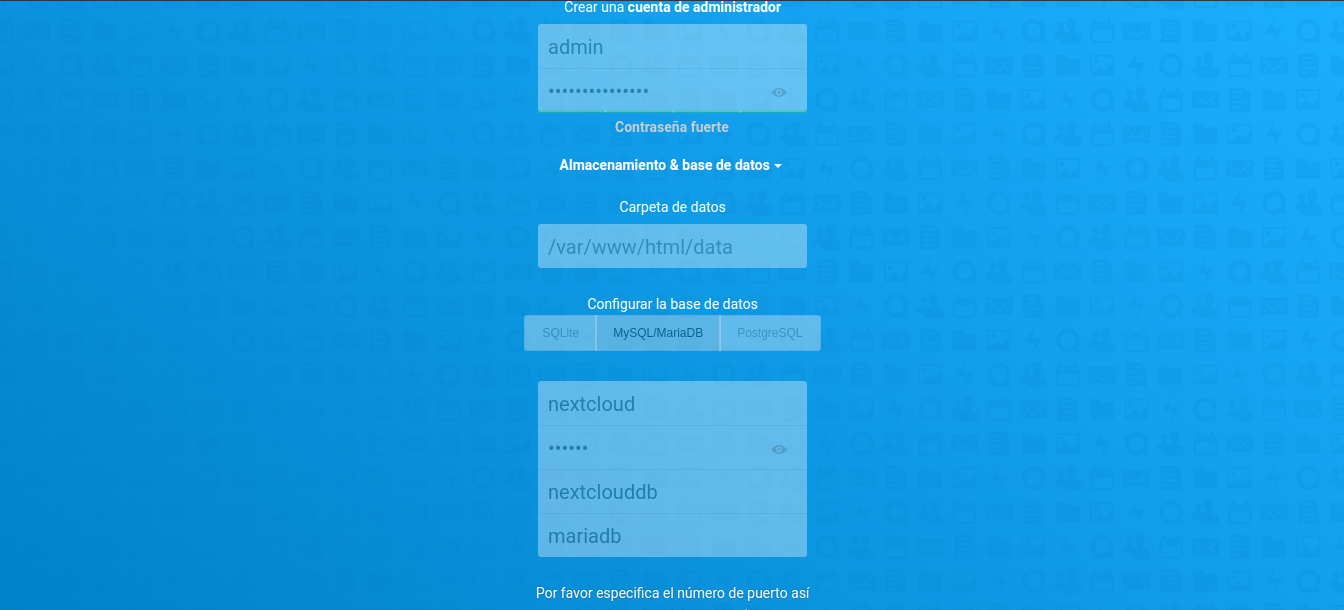
\includegraphics[width=0.9\textwidth]{imagenes/docker/nextcloud/configurarNextcloud.png}
				
				\caption{Configurar Nextcloud}
				
				\label{fig:nextcloud}
				
			\end{figure}
			
			\pagebreak
			
			\begin{tcolorbox}[enhanced,frame style image=blueshade.png,opacityback=0.75,opacitybacktitle=0.25, colback=blue!5!white,colframe=blue!75!black,title=Nextcloud]
				Para acceder a NextCloud en el navegador se debe colocar la dirección IP del servidor Docker y el puerto donde escucha el contenedor. En mi caso seria \href{http://192.168.1.222:8080/}{\color{blue}http://192.168.1.222:8080}
			\end{tcolorbox}
			
			Finalizada la configuración y ya dentro del dashboard me dirigiré al perfil del usuario administrador, donde podre crear los usuarios que tendrán acceso al servicio de Nextcloud.
			
			\begin{figure}[ht]
				
				\centering
				
				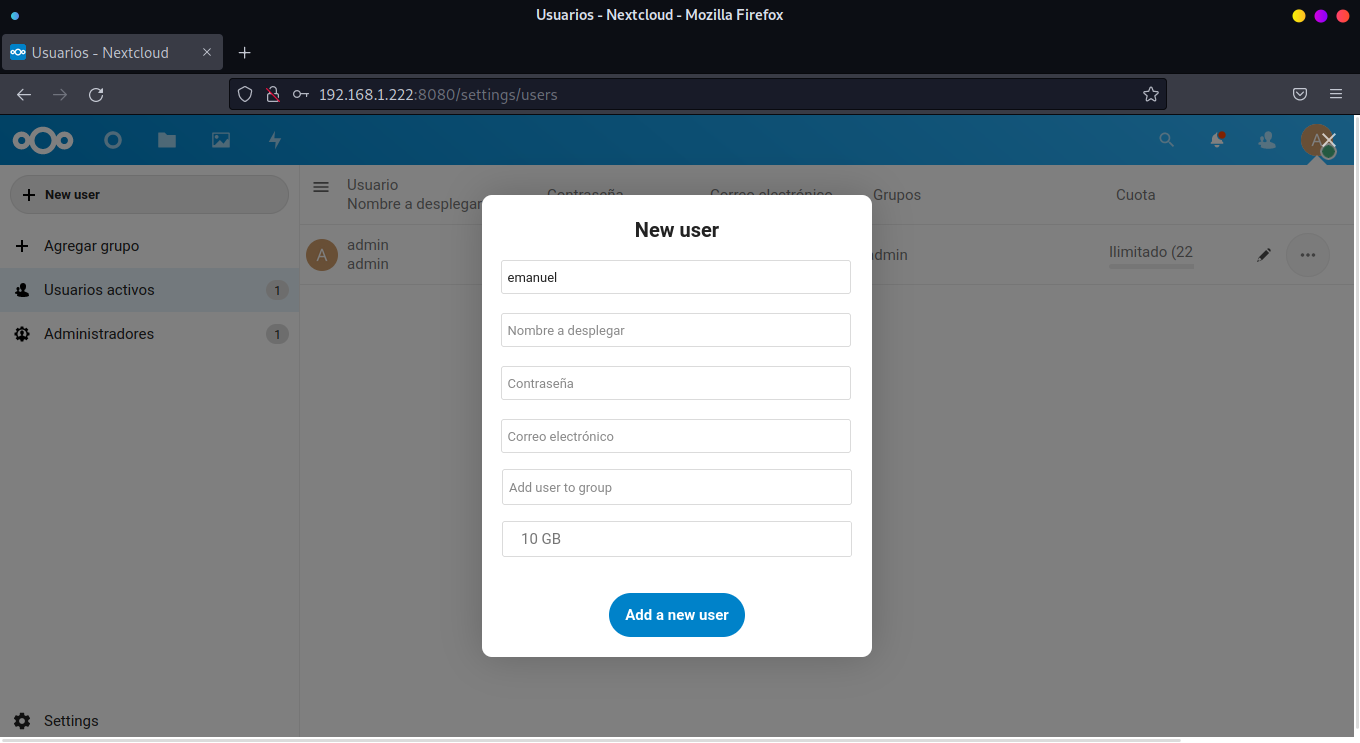
\includegraphics[width=0.9\textwidth]{imagenes/docker/nextcloud/creacionUsuarios.png}
				
				\caption{Creación de Usuarios}
				
				\label{fig:usuarios}
			\end{figure}	
		
		Los alumnos podrán hacer uso de este servicio solamente desde la red lan a través de un navegador web. Donde cada uno accederá con su usuario y contraseña.\par
		
		\subsection{Conclusión}
			
			Con Nextcloud la información se almacena de forma segura en un lugar controlable. NextCloud replicar las capacidades de servicios externos de almacenamiento en la nube, permitiendo compartir contenido entre usuarios de la misma red local.

	\section{Contenedor Emby}
	
		\subsection{¿Que es Emby?}
		
			Emby es un centro de multimedia multiplataforma que permite visualizar contenido desde cualquier tipo de dispositivo via Web, App o DLNA. 
		
			Emby trabaja con el contenido multimedia almacenado en servidor local, esto lo hace ideal dadas las características del Aula Virtual.\par
			
		\subsection{Características de Emby:}
			
			\begin{itemize}
				
				\item El servidor de Emby convierte y envía automáticamente los vídeos a cualquier dispositivo.
				
				\item Cuenta con canales de vídeo en directo.
				
				\item Permite sincronizar librerías con los clientes móviles.
				
				\item La organización está muy cuidada para ser sencilla de ver y entender.
				
				\item Cuenta con controles parentales.
				
				\item Servidor DLNA para reproducir el contenido multimedia.
				
				\item Compatible con Chromecast.
	
			\end{itemize}
		
		\subsection{¿Qué es un centro multimedia?}
		
			Un centro multimedia es una aplicación que gestiona el contenido multimedia (fotografías, musica y vídeos), para que se pueda reproducir en el mismo dispositivo donde esta almacenado o en otros dispositivos, en este caso, conectados a la red LAN.
		
			Emby, cuentas con la aplicación servidor que gestiona el contenido y lo transmite por streaming, y por otro lado la aplicación que recibe el contenido. La cual puede ser el cliente que se encuentra disponible para la plataforma de Windows, Mac, Linux, FreeBSD, dispositivos NAS, Android, iOS, Windows Phone, Android TV, Fire TV, Apple TV, Kodi, Xbox, etc. O  cualquier navegador compatible con HTML5.
		
		\subsection{Preparación del área de trabajo}
			
			Mi directorio de trabajo sera /srv donde creare un directorio que almacenara toda las configuraciones de Emby.\par
			
			\begin{lstlisting}[language=Bash,caption=Directorio de trabajo Emby]
				#cambiar al directorio srv
				cd /srv
				#crear directorio
				mkdir emby
				#cambiar directorio
				cd emby
			\end{lstlisting}
			
			\clearpage
			
			Dentro del directorio creare un documento docker-compose.yaml el cual contendra el siguiente codigo:
								
			\inputminted{yaml}{documentos/docker/emby/docker-compose.yml}
			
			\begin{tcolorbox}[enhanced,attach boxed title to top center={yshift=-3mm,yshifttext=-1mm},
			colback=blue!5!white,colframe=blue!75!black,colbacktitle=red!80!black,title= Estructura del documento,fonttitle=\bfseries, boxed title style={size=small,colframe=red!50!black} ]
			
			\centering
			
				Descripción del código \ref{estructura-docker}
			
			\end{tcolorbox}
			
			\subsection{Crear Contenedor Docker:}\par\vspace{0.2cm}
			
			\begin{lstlisting}[language=bash,caption=Crear contenedor Docker]
	
				docker-compose up -d
			\end{lstlisting}	
			
			\subsubsection{Explicación del comando anterior:}\par
			
			\begin{itemize}
				
				\item \textbf{docker-compose:} Define y ejecute aplicaciones de varios contenedores con Docker.
				
				\item \textbf{up:} Crea e inicia el contenedor.
				
				\item \textbf{-d:} Ejecuta contenedores en segundo plano.
				
			\end{itemize}
			
			Este proceso puede demorar varios minutos, dependiendo de la velocidad de la conexión al Internet con la que se cuente. Una vez finalizada la descarga de la imágene se ejecutara el contenedor.\par
	
		\subsection{Configuración Emby}
					
			Una vez que el contenedor se encuentra en ejecución me dirigiré al navegador web para terminar de realizar las configuraciones. Al igual que en NextCloud, para acceder al servicio de Emby solo se debe colocar en el navegador web la dirección IP del servidor Docker y el puerto donde escucha. En mi caso seria \href{http://192.168.1.222:8096/}{\color{blue}http://192.168.1.222:8096}
			
			\begin{itemize}
				
				\item \textbf{Idioma:} Seleccionar el lenguaje de la Interfaz Emby.
				
				\item \textbf{Crear usuario y contraseña:} Creación del usuario para acceder a la interfaz web de Emby.
				
				\item \textbf{Agregar Contenido Multimedia:} Seleccionar los directorios donde se encuentran todo el contenido multimedia que se compartirá con la red lan.
				
				\item \textbf{Lenguaje de las Bibliotecas:} Seleccionar el Lenguaje con el que se mostrara la información del contenido multimedia en la plataforma web.
				
				\item \textbf{Términos y Condiciones:} Aceptar los términos y condiciones de Emby.
				
				\item \textbf{Final de Configuración:} Ahora Emby se encargara de realizar las demás configuraciones, mientras ofrece los clientes de todas las plataformas soportadas.
				
				\item \textbf{Login:} Ingresar al sistema web.
				
			\end{itemize}
		
			\subsubsection{Panel de control de Emby}
			
				\begin{figure}[ht]
					
					\centering
					
					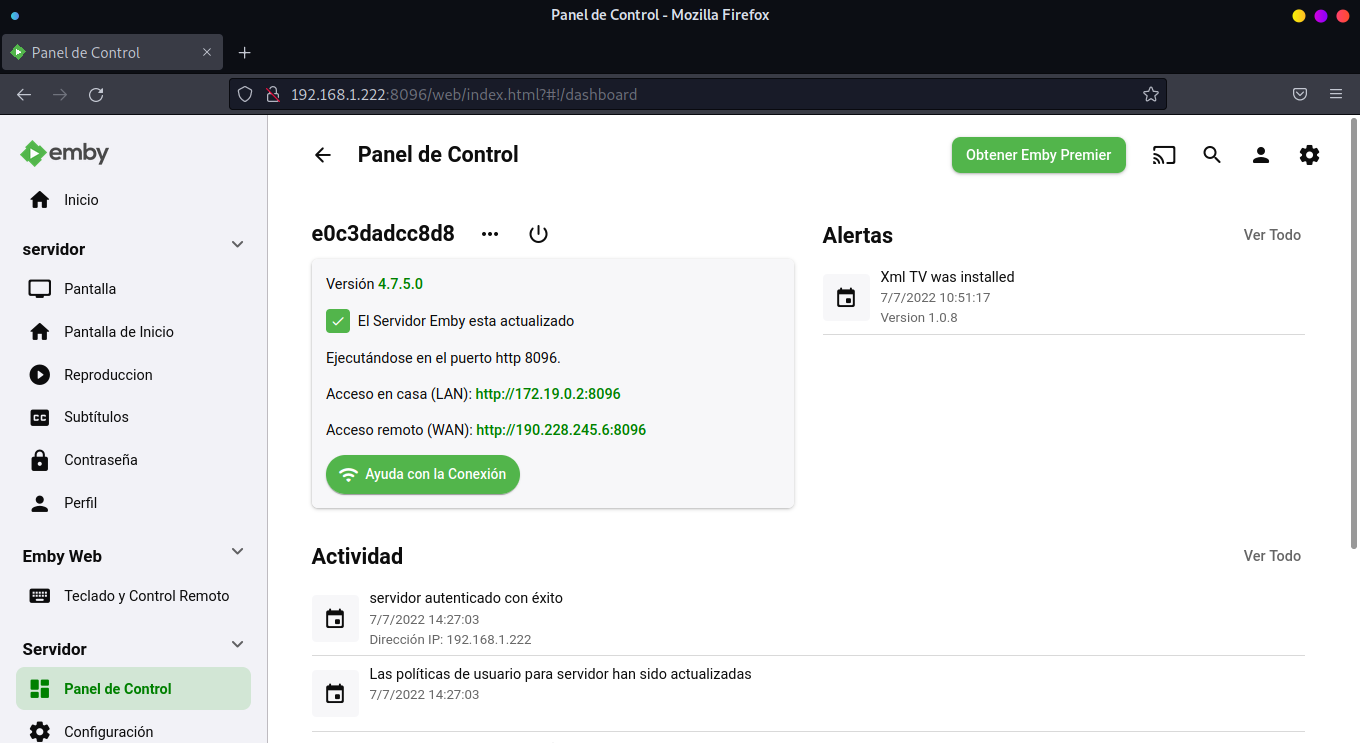
\includegraphics[width=0.9\textwidth]{imagenes/docker/emby/emby-dashboard.png}
					
					\caption{Dashboard}
					
					\label{fig:dashboard}
					
				\end{figure}
					
		\subsection{Conclusión}
		
			Uno de los problemas que tenemos en el Aula virtual es la velocidad de conexión al Internet (2MB). Lo que dificulta en gran manera la reproducción de Vídeos Tutoriales o contenido multimedia recomendado por los docentes.\par
			
			Ahora se descarga el contenido multimedia y se almacena de forma segura en un lugar controlable dentro del Servidor Local y con Emby por medio de streaming se comparte con toda la red lan.\par
	
